El almacenamiento de votos es importante a corto y largo plazo. Es necesario poder obtener un resultado correcto al momento de finalizar la elección, pero también deben estar disponibles los datos si se quisiera hacer un recuento en el futuro.
Por lo visto, no hay una única forma de almacenar los votos durante el sufragio y se utilizan diversas formas para ello. Desde distintos medios de almacenamiento como tarjetas RFID hasta la propia memoria de la máquina de votación, donde no necesariamente es excluyente alguna de las dos.
A continuación distintas técnicas que se utilizaron en distintos países, y los agujeros de seguridad que se encontraron en cada una.

\subsection{Máquinas con almacenamiento en memoria}

Como primero ejemplo, en Estados Unidos se utilizó la terminal de votación AccuVote TSX, por más de 12 millones de votantes en más de 350 jurisdicciones en los Estados Unidos. Los votos son almacenados en una tarjeta PCMCIA.\footnote{\url{http://www.engr.uconn.edu/~sad06005/pubs/Conference/sac12.pdf}}
%En el paper mencionado, cuenta que para emitir votos de forma electrónica se utilizó la terminal de votación AccuVote TSX, utilizada por más de 12 millones de votantes en más de 350 jurisdicciones en los Estados Unidos. Los votos son almacenados en una tarjeta PCMCIA.

Esta terminal tiene vulnerabilidades que permiten un ataque que intercambia los votos de dos candidatos y otro que borra el nombre de un candidato. Ambos ataques son capaces de eludir las comprobaciones de integridad de cifrado implementados en la terminal. Los ataques se pueden iniciar en cuestión de minutos y sólo requieren una computadora con la capacidad para montar una tarjeta PCMCIA. No es necesario que el atacante tenga información de la elección que va a modificar, sólo es necesario que tenga acceso a la maquina de votación para abrir el compartimiento donde se almacena la tarjeta PCMCIA.

Las vulnerabilidades encontradas en una auditoría fueron:
\begin{itemize}
	\item Aunque el nombre de cada candidato está acompañado por 128 bits de integridad, la terminal no los usa de forma efectiva. Cuando falla el chequeo de integridad en un candidato, no se cuenta el voto para este candidato. Aunque el elector verifique en la boleta VVPAT que figura el candidato de forma correcta, su voto no será tenido en cuenta para el recuento de votos ya que el recuento electrónico lo realiza con lo almacenado en la tarjeta PCMCIA y al fallar la integridad del candidato, no lo cuenta. Tampoco existe una verificación de la integridad de que no se cambió los nombres de candidatos en los recuentos de los votos
	\item No hay una firma criptográfica de la tarjeta PCMCIA. Por ende, se puede agregar más contenido a la urna de votación
	\item La existencia de puertas traseras como en versiones anteriores de la terminal y un mecanismo de actualización de archivos débil, ya que tan solo se utiliza el nombre del archivo a actualizar para identificar una actualización de software válida
	\item Las máquinas de votación tienen todas la misma llave física para obtener la tarjeta PCMCIA, al menos en las que fueron revisadas
\end{itemize}

De este modo, se tiene un recuento de votos en un medio vulnerable a ataques, por varios medios; y cuyas medidas de seguridad no permiten auditar la corrección del contenido, con lo que podría ser modificable y pasar desapercibido a menos que se realizase una auditoría incluyendo los registros en papel. Por otro lado, la mera utilización de herramientas criptográficas puede conducir a una falsa sensación de seguridad. Con el fin de ser eficaz, la criptografía debe ser utilizada en conjunción con un buen diseño que proporcione una protección completa en la integridad de la información crítica.
% \subsection{Estados Unidos}
% En este país encontramos un caso que nos llama la atención ya que se utiliza criptografía en el voto electrónico, pero no es utilizada correctamente. Como dice el paper
% \footnote{\url{http://www.engr.uconn.edu/~sad06005/pubs/Conference/sac12.pdf}}
% que leímos sobre esta votación, la mera utilización de herramientas criptográficas puede conducir a una falsa sensación de seguridad. Con el fin de ser eficaz, la criptografía debe ser utilizada en conjunción con un buen diseño que proporcione una protección completa en la integridad de la información crítica.

También en Estados Unidos, pero en otro estado
\footnote{\url{http://usatoday30.usatoday.com/news/politicselections/vote2004/2004-11-04-votes-lost_x.htm}}
 utilizando el voto electrónico, fue que más de 4.500 votos se perdieron en un condado de Carolina del Norte, porque las autoridades creían que una máquina de votación electrónica podía contener más datos que los que efectivamente almacenaba. Es difícil encontrar detalles técnicos que describan lo que sucedió, ya que principalmente fueron los medios los que hablaron de eso, pero se supone que los fabricantes no avisaron o dieron un número incorrecto de votos que la máquina podía almacenar, y en el condado usaron una sola máquina para toda la votación de un espacio de tiempo (llamado ``early voting'').

En otro ejemplo de Estados Unidos, pero en Connecticut, hay máquinas ($https://www.usenix.org/legacy/events/evt08/tech/full_papers/davtyan/davtyan_html/index.html$) que guardan toda la información de la elección, desde la ``configuración'' de la elección como candidatos, hasta los resultados tabulados en memorias externas que son enviadas a una ubicación central para el conteo final.
% HABRIA QUE EXPANDIR UN TOQUE MAS

\subsection{Almacenamiento externo}

Otra forma de almacenar los votos, es la implementada en las elecciones del 2015 en Argentina y en las elecciones previas al 2010 en Israel, donde los votos se graban en un chip RFID que se encuentra en la boleta (En el caso de Argentina sería la BUE) y se deposita la boleta en una urna física. Luego, en el escrutinio de votos, se utiliza una máquina para leer la información de la boleta y poder contabilizar el voto. 

Según la auditoría realizada por la ITBA para la Defensoría del Pueblo de la C.A.B.A
\footnote{\url{http://www.defensoria.org.ar/wp-content/uploads/2015/06/InformeAudotoriaVotoElectronico.pdf}}
, existen tres posibles problemas al retirar la BUE:
\begin{itemize}
	\item Si la máquina ha iniciado la grabación del chip RFID pero no la ha finalizado, el sistema ya no responde y se tiene la necesidad de reiniciar la máquina
	\item Si la máquina ha finalizado la grabación del chip RFID, entonces queda una boleta con el voto registrado sólo en el chip RFID, sin el voto impreso en la boleta
	\item Si la máquina ni siquiera ha iniciado la grabación del chip RFID, entonces al volver a ingresar para un nuevo voto, en la pantalla se muestra la selección del votante anterior en un recuadrado en verde
\end{itemize}


En la sección de privacidad, seguiremos mencionando estos países ya que los comentarios acerca de los posibles ataques tienen más que ver con la pérdida del anonimato que con el formato de almacenamiento en sí.

\subsection{Mal uso de esquemas de encriptación}
Analizando el sistema de votación electrónica de Brasil, se observan dos problemas mencionados a continuación respecto a la encriptación utilizada en el sistema.
\footnote{\url{https://ivan.barreraoro.com.ar/wp-content/uploads/2015/09/Software-vulnerabilities-in-the-Brazilian-voting-machine.pdf}}
\begin{itemize}
	\item \textbf{Algoritmos de encriptación obsoletos:} La función criptográfica SHA-1 utilizada para computar firmas digitales y chequeos de integridad no es resistente a colisiones. Un ataque aprovechando esta vulnerabilidad podría permitir a un atacante construir un software de votación malicioso capaz de producir resultados falsos indistinguibles de los resultados correctos.
	\item \textbf{Uso inadecuado de encriptación: } La misma clave de encriptación es compartida por todas las terminales de votación. Esta clave es utilizada para encriptar sus tarjetas de memoria de almacenamiento. Para empeorar las cosas, la clave criptográfica tambien esta guardada en texto plano en las memorias de almacenamiento. Claramente esta es una vulnerabilidad a la confidencialidad de la información.
\end{itemize}


\subsection{Falta de seguridad respecto a la configuración y mantenimiento del SO}
En un informe publicado por VITA \footnote{(VIRGINIA INFORMATION TECHNOLOGIES AGENCY)} acerca del sistema de voto electrónico en Virginia, USA, se menciona que el sistema utilizado en las terminales de votación era un Windows XP Embedded 2002 sin los ultimos parches de seguridad, cosa que permitía explotar vulnerabilidades conocidas. Particularmente, se realizó un ataque al file-sharing system utilizando fuerza bruta para adivinar la password de acceso de Administrador, utilizando un simple diccionario concluyeron que la password era ``admin'', permitiendo acceso a los siguientes servicios de la terminal:

\begin{itemize}
	\item Remote Desktop Protocol: Podia accederse remotamente como administrador a la terminal de voto.
	\item Los paths compartidos por defecto como ``\$C'', ``\$D'', ``ADMIN\$'', etc eran accesibles para la transferencia de datos.
\end{itemize} 

Junto a esto, cada terminal poseía una base de datos \texttt{Microsoft Access} conteniendo información sensible como ser la información de dicha terminal, la ubicación y el numero de votos. Dicha base estaba protegida por una password tan debil que fue crackeada en 10 segundos utilizando una herramienta para tales fines.
Unificando estas debilidades mencionadas, sumadas a la pobre seguridad en la red Wifi de las terminales\footnote{Mas de esto en transmisión}, constituyen un espectacular ataque en el cual se puede reemplazar la base de datos de votación de la terminal manteniendose cerca y accediendo mediante red Wifi.\footnote{\url{https://www.schneier.com/blog/archives/2015/04/an_incredibly_i.html}}.

%%% PASADO A SEG FISICA
% El componente electrónico de votación en India, llamado EVM, está compuesto por dos partes: la unidad de votación (izquierda) y la unidad de control (derecha) que están enlazadas por un cable de 5 metros. Las unidades de votación están realizadas para soportar hasta 16 candidatos. En caso de ser más candidatos, se agrega otra unidad de votación y es posible agregar hasta 4 unidades de votación, dando una capacidad máxima de 64 posibles candidatos. En la unidad de votación, se agrega una hoja indicando que botón representa a cada candidato con el símbolo de su partido político. Para votar, el elector tiene que ser identificado por el presidente de mesa que luego le realiza una marca en el dedo con tinta indeleble para evitar que vuelva a votar y presiona un botón en la unidad de control, permitiendo al elector votar en la unidad de votación. Al realizar esto, se prende una luz en la unidad de votación indicando que el votante está listo para sufragar.

% \begin{figure}[h]
% 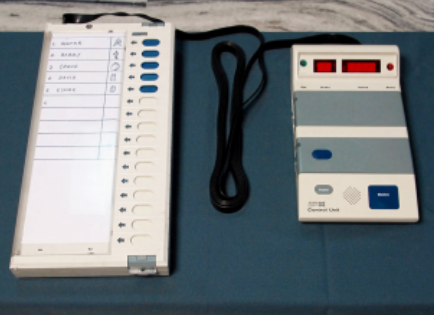
\includegraphics{Imagenes/almacenamiento1}
% \caption{Máquina de votación electrónica utilizada en India}
% \end{figure}

% Las vulnerabilidad encontrada en el paper leído es
% \footnote{\url{https://jhalderm.com/pub/papers/evm-ccs10.pdf}}
% que se puede reemplazar fácilmente algún componente del equipo sea CPU, placas o agregar hardware. Los diseñadores de las EVM podrían haber hecho los ataques más difíciles agregando un mecanismo criptográfico para identificar a los distintos componentes de hardware originales, como un mecanismo de challenge response basado en un secreto contenido en el firmware original.

% Uno de los posibles ataques mencionados en el paper es Dishonest Display. Se desarrolló una placa de visualización que puede reemplazar a la placa real en la unidad de control. Normalmente, cuando los votos son contados, la cantidad de votos recibidos por cada candidato figura en el tablero real. Con el ataque, el tablero agrega un microcontrolador que intercepta los votos totales y realiza la sustitución fraudulenta de resultados emitiéndose en el tablero de visualización. Notar que en este ataque hay que realizar un intercambio de un componente de hardware.

% \begin{figure}[h]
% 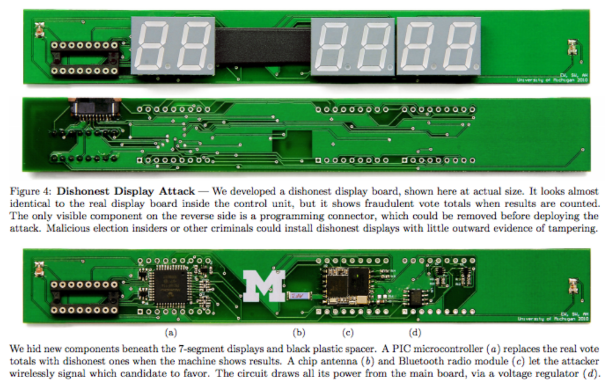
\includegraphics[width=0.8\textwidth]{Imagenes/almacenamiento2}
% \caption{Hardware utilizado}
% \end{figure}

% %Además, el paper menciona otro ataque más pero optamos comentarlo en la sección de privacidad ya que tiene más relación con la pérdida del anonimato.
% Un detalle no menor, es que el recuento de votos de la elección en India se realiza semanas después del sufragio. Por ende, el atacante tiene tiempo para poder realizar el cambio o agregar hardware que le permite realizar el ataque mientras están almacenadas.

% \subsection{Holanda}
% Este país
% \footnote{\url{https://www.ndi.org/e-voting-guide/netherlands-CS/opposition-to-e-voting}}
% \footnote{\url{http://wijvertrouwenstemcomputersniet.nl/English}}
%  nos llamó la atención porque debido la fuerza mediática que tuvo en la sociedad la difusión de un video
% \footnote{\url{http://www.veoh.com/watch/v505707dgewqMsB}}
%  sobre las máquinas de votación NEDAP podían ser manipuladas, se logró volver a votar en papel y lápiz, como se votaba anteriormente en este país.
% Sucedió algo similar al caso de India: se necesitaban 5 minutos para poder manipular una de estas máquinas NEDAP cambiando dos chips, y como estas estaban guardadas sin una seguridad correspondiente al tema en cuestión, cualquier persona podia modificarlas.

